\chapter{Experiment 2}

\textbf{Author: Peter Kain} 

The second experiment is performed for the reason of testing the neural network with images of real objects. This experiment is mandatory for testing the capabilities of the neural network when it comes to real images.

\section{Preparation}
The first step of the authors was choosing a suitable object. In an effort to be time efficient once again the monkey head was chosen. This had the advantage that 3D-printing the object was easy, as all the authors had to do was exporting the existing model from Blender, and, even better, the trained weights of this object were already existing. Next the 3D model of the head was modified to include a cylindrical hole at the bottom, be able to easily mount the object. The last step was printing the object with a 3D printer. For this a Ultimaker Original and pink PLA (Polylactic acid) filament was used.

\section{Setup and Environment}
The setup consisted of a Parrot Bebop 2 and the 3D printed monkey head put on a stick to simulate the height of the head in the images produced by Blender. The authors chose a mostly white background, consisting of a table and a painted wooden board leaned on the table.

The authors were not specific about the lighting, because this experiment was to be performed as realistic as possible. For example in drone competitions the lighting often can not be influenced.

The monkey head was placed on the table facing away from the white wooden board. The drone was positioned at a distance of approximately 14cm from the object. The drone's camera was looking directly towards the object. After taking the first image the drone was moved to a second position, again about 14cm away and looking at the object. This resulted in the drone rotating slightly to the left to keep the object centred.

The images were taken with Parrot SA's FreeFlight Pro app.

\section{Sequence of Events}
The two images taken with the drone's camera from the different positions then had to be modified in order to be recognized by our neural network. The main differences between these images and the Blender generated ones were the different aspect ratio and a distortion, caused by to the way the camera operates. This can be seen in Figure~\ref{pic:experiment2_environment_comparison}. The authors wanted to make the images in (a) look like the images in (b), so modifications were necessary. The following modifications were executed with the program GIMP (GNU Image Manipulation Program), as the authors had previous experience with it:

First, the authors had to rotate the images to the left by 90 degrees, since the original images were saved in landscape. Then the authors needed to modify the aspect ratio, were cropping the image came into play. After cropping the image the final step was to get rid of the distortion. This is was relatively easy as GIMP already has a built-in distortion filter. After reversing the existing distortion the result can be seen in (c), which can then be used by our neural network to predict the distance to the drone.

Lastly the authors feed the final, undistorted images into the Neural Network, with the trained monkey head weights loaded.

\begin{figure*}[h!]
	\centering
	\begin{subfigure}[t]{\textwidth}
		\centering
		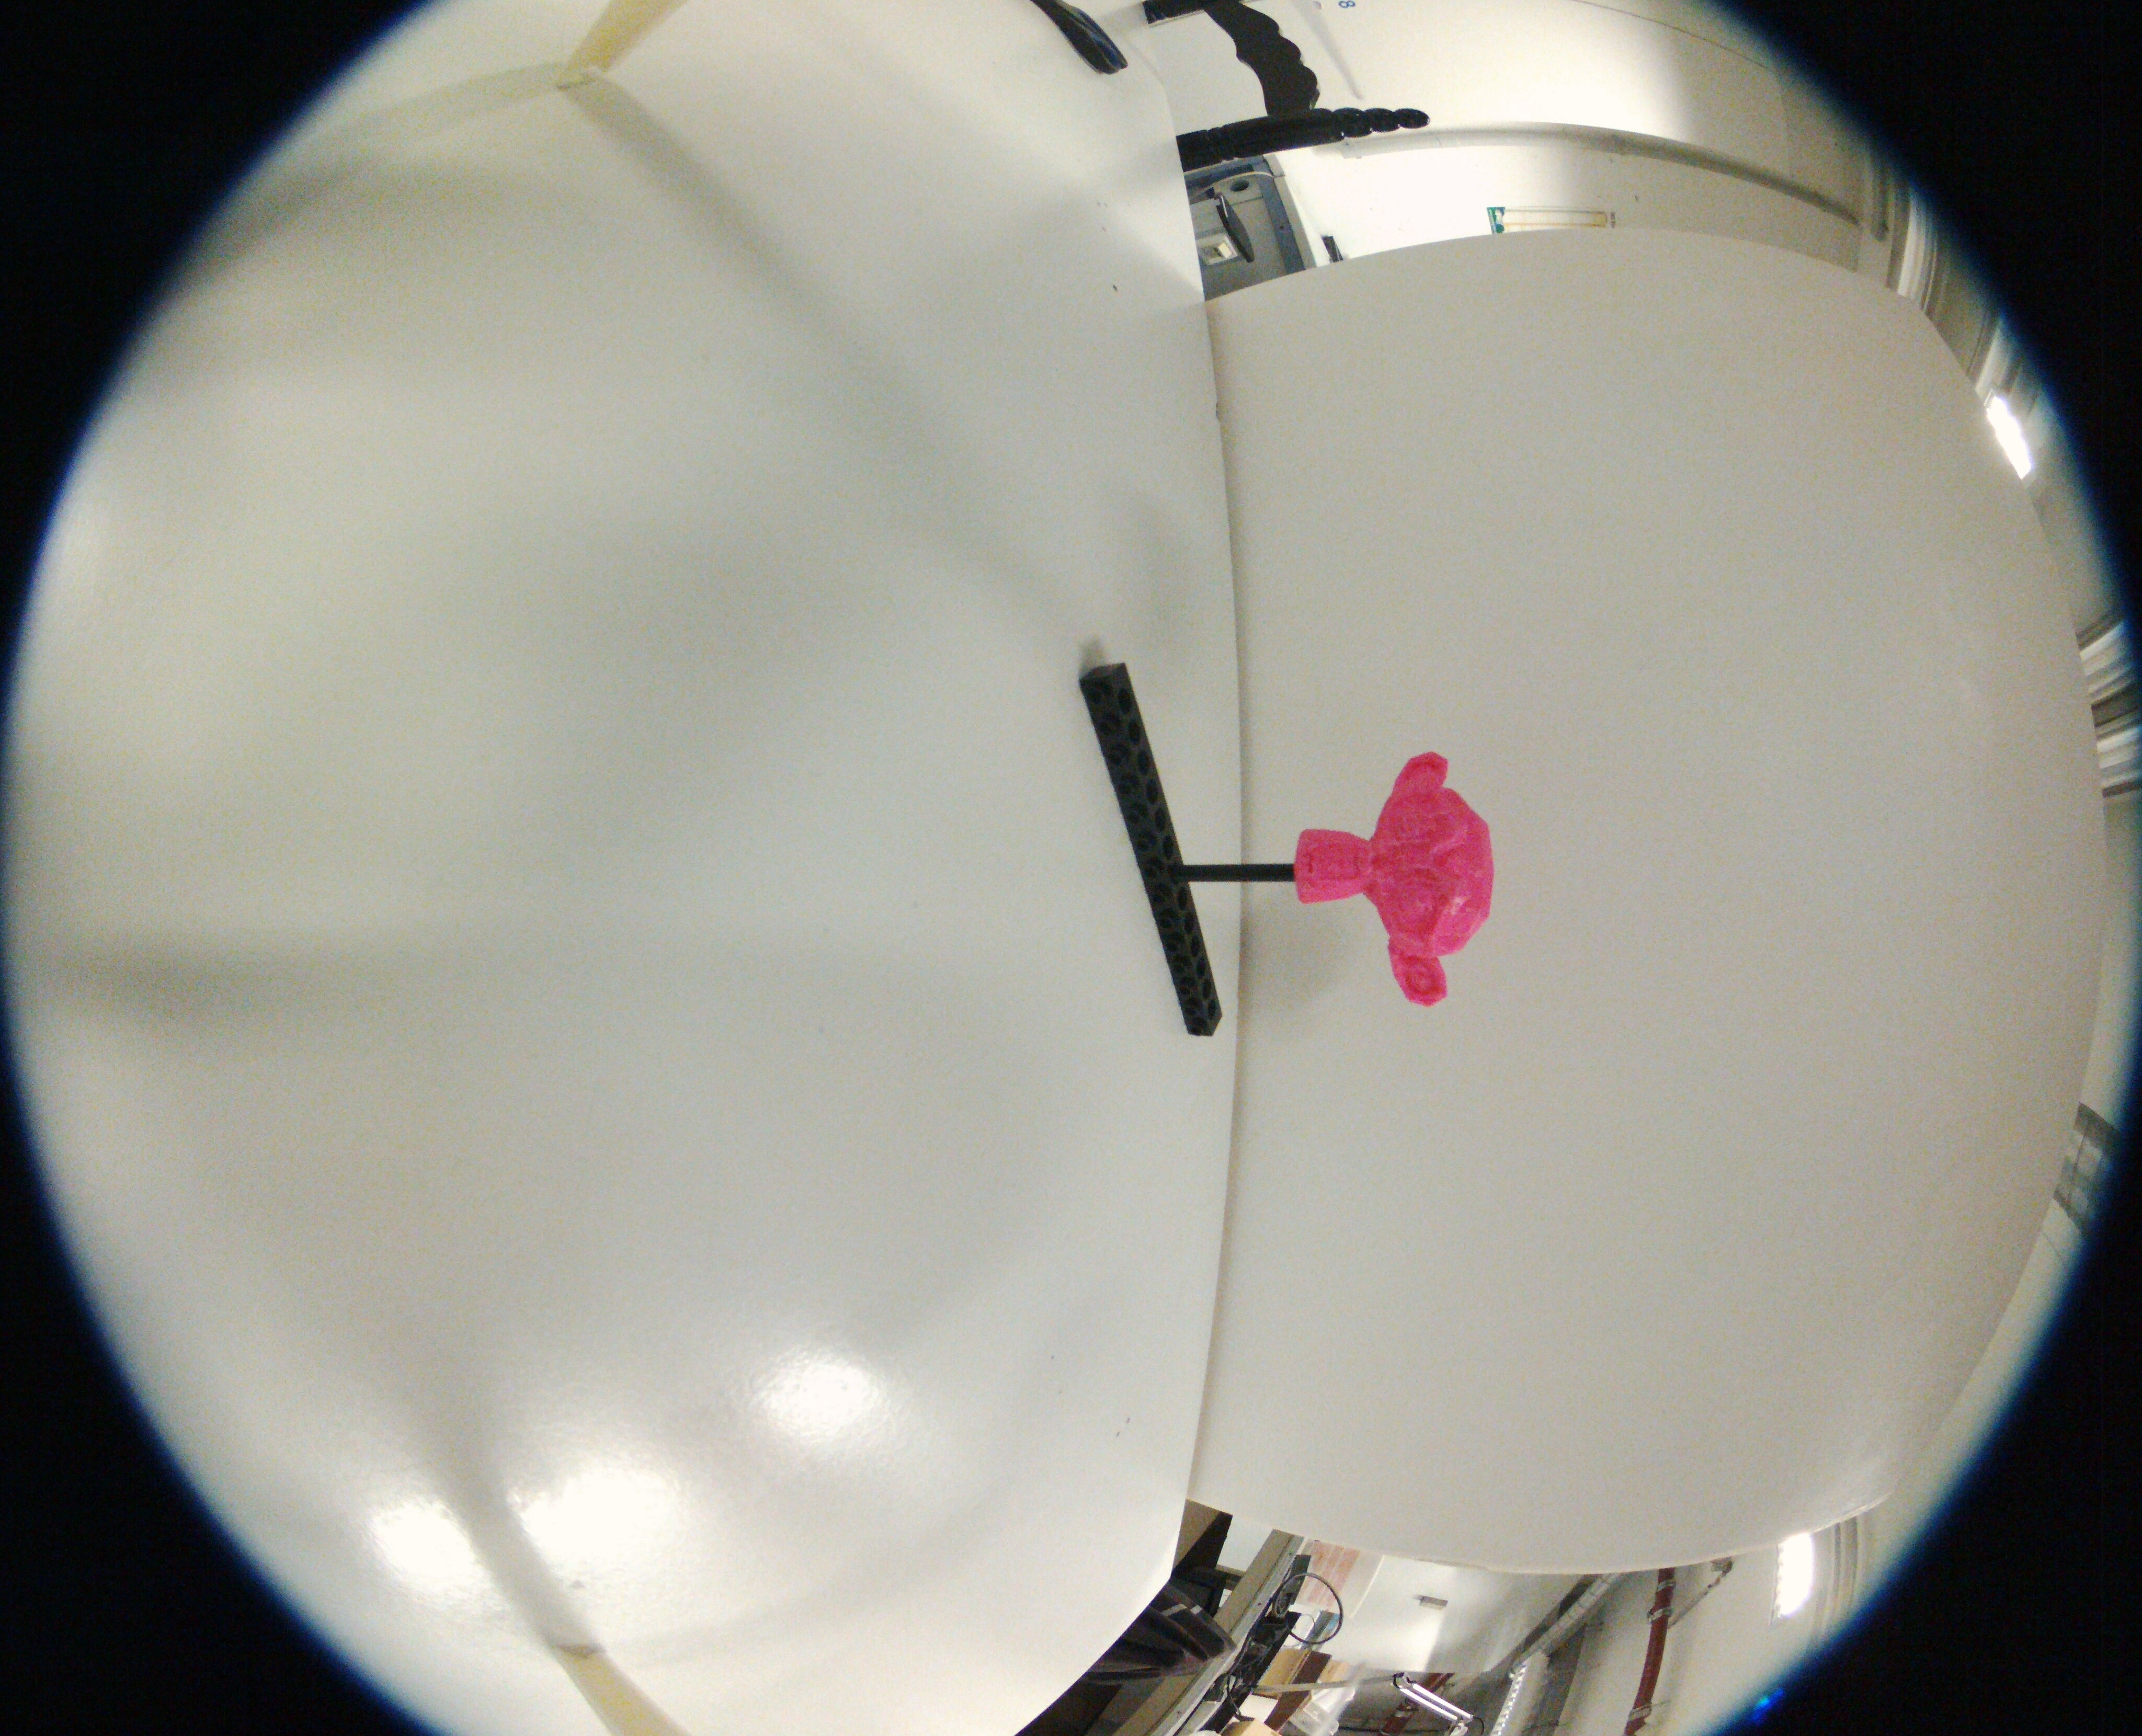
\includegraphics[width=0.48\textwidth]{img/experiment1_original_bebop_img_1.jpg}
		\hfill
		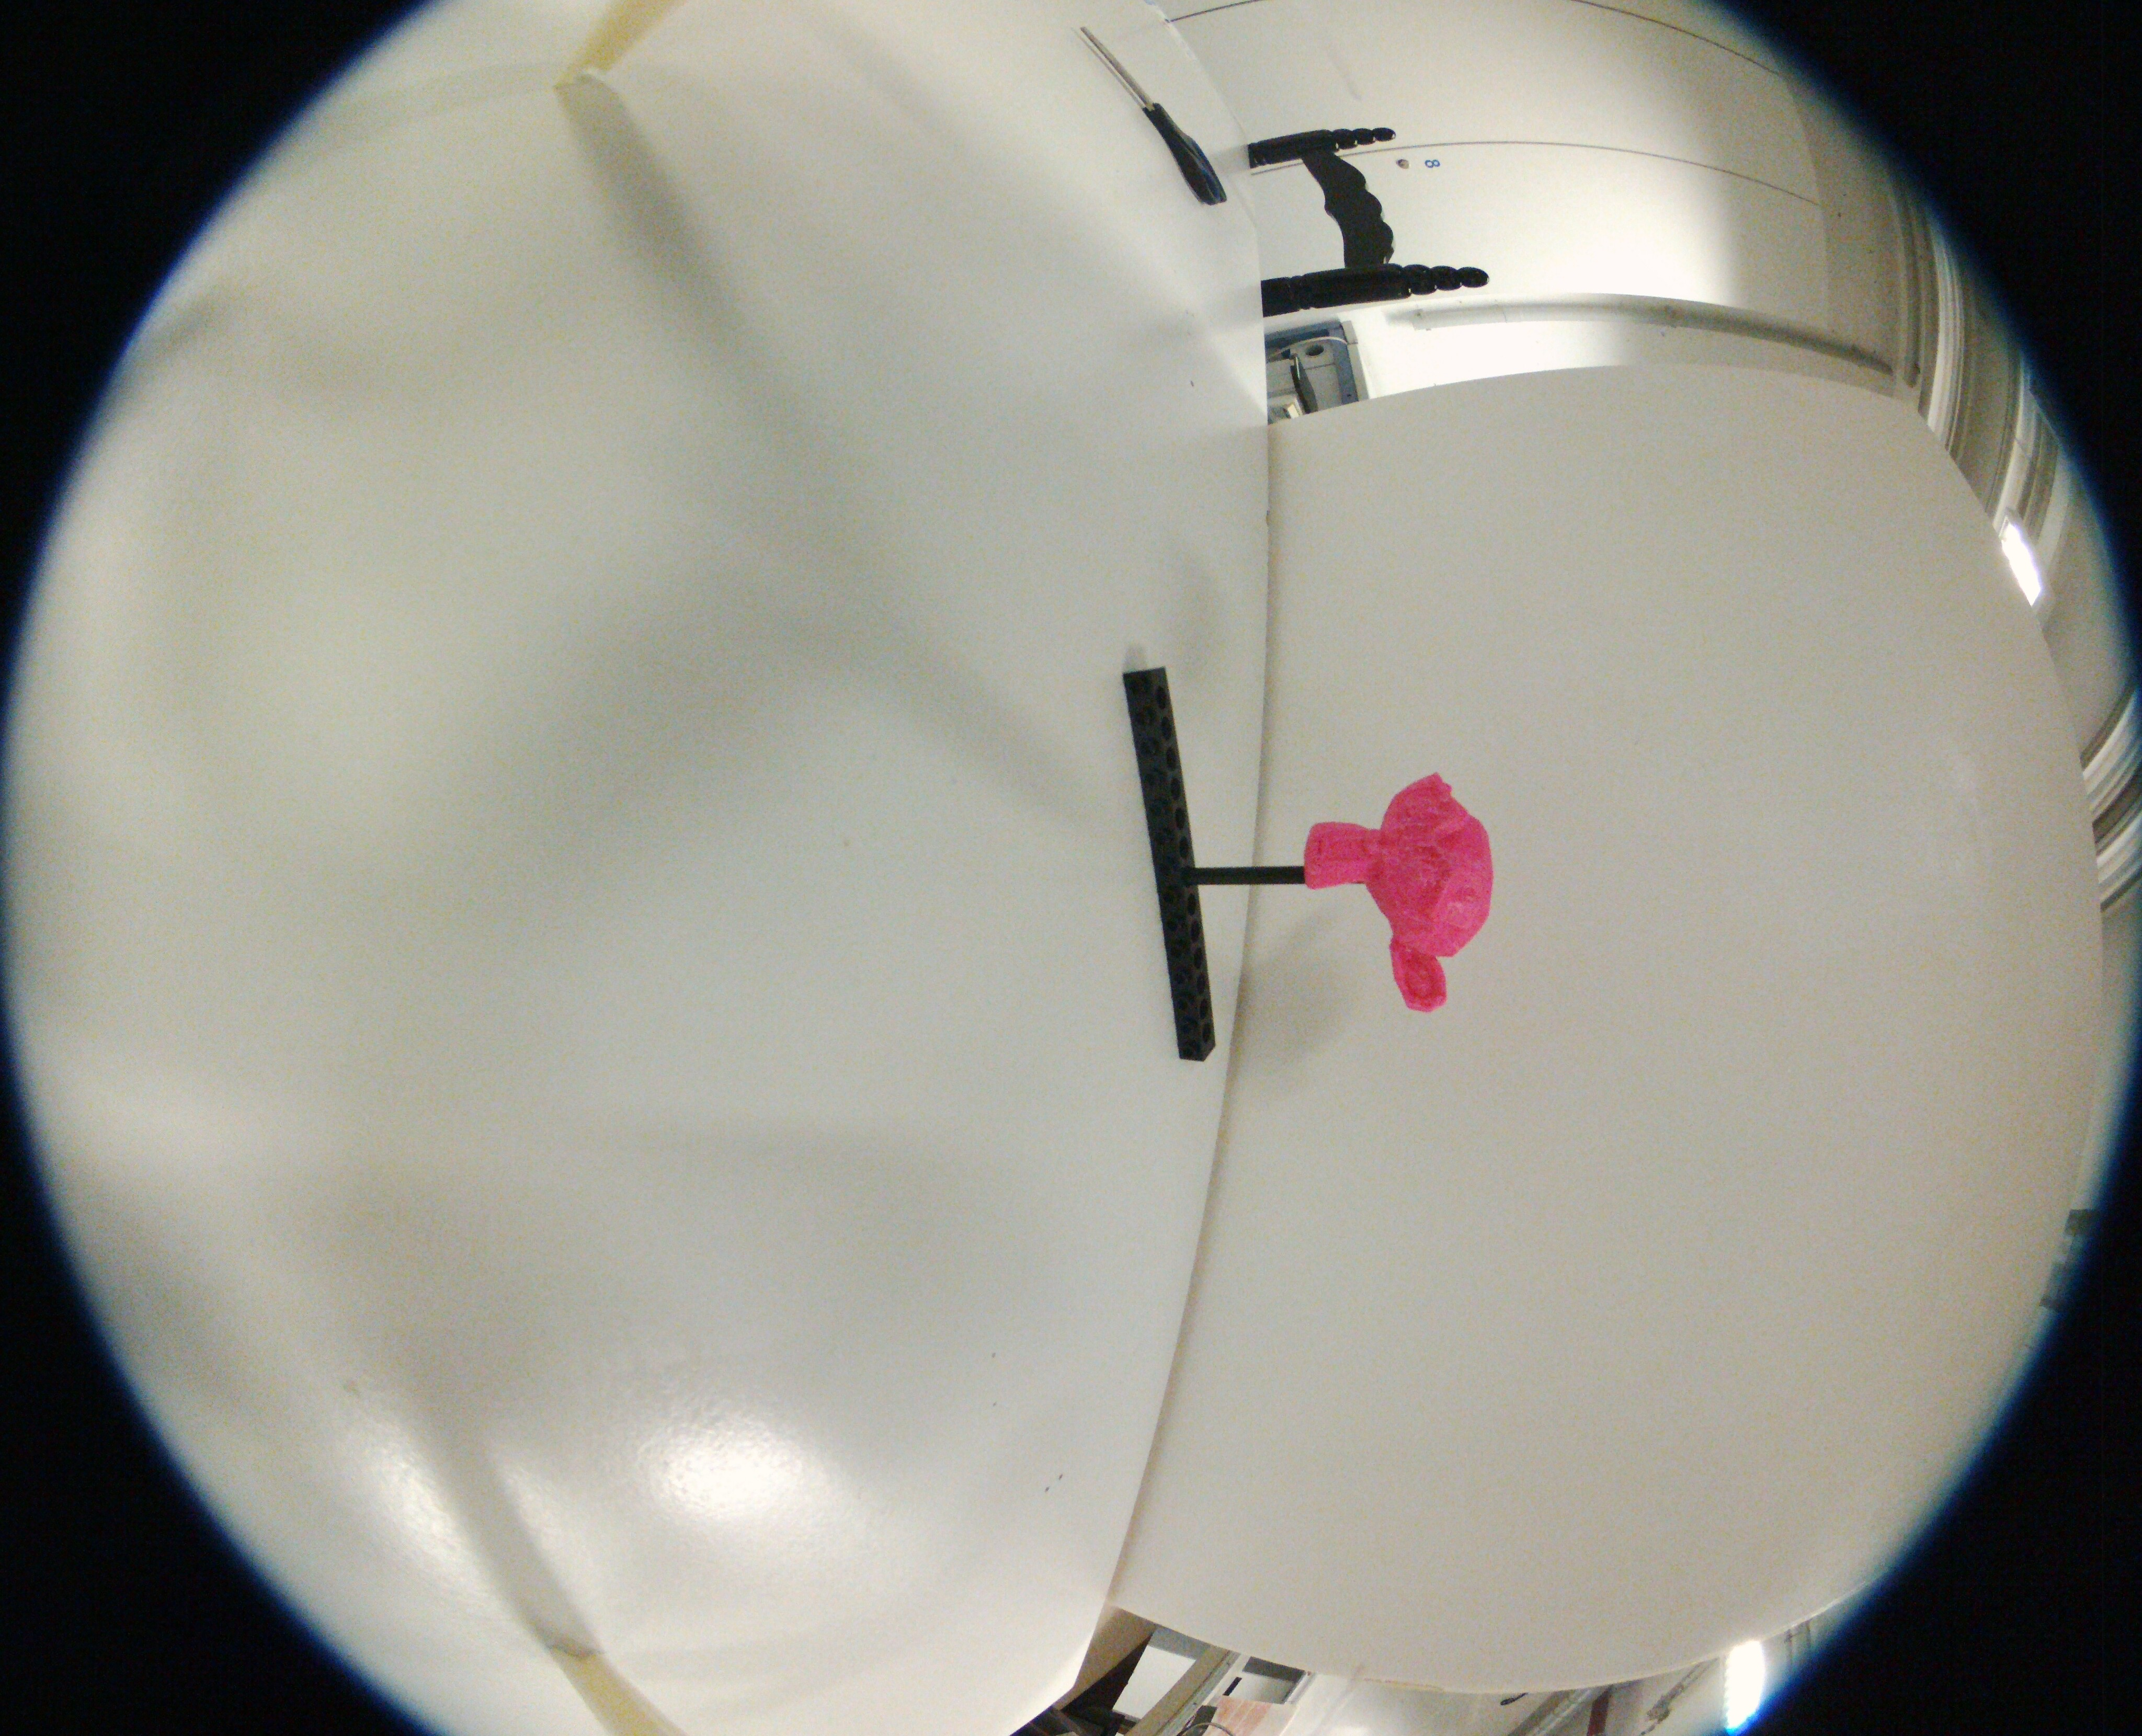
\includegraphics[width=0.48\textwidth]{img/experiment1_original_bebop_img_2.jpg}
		\caption{The original images of the 3D printed monkey head produced by the Parrot~Bebop~2.}
	\end{subfigure}
	~ 
	\begin{subfigure}[t]{\textwidth}
		\centering
		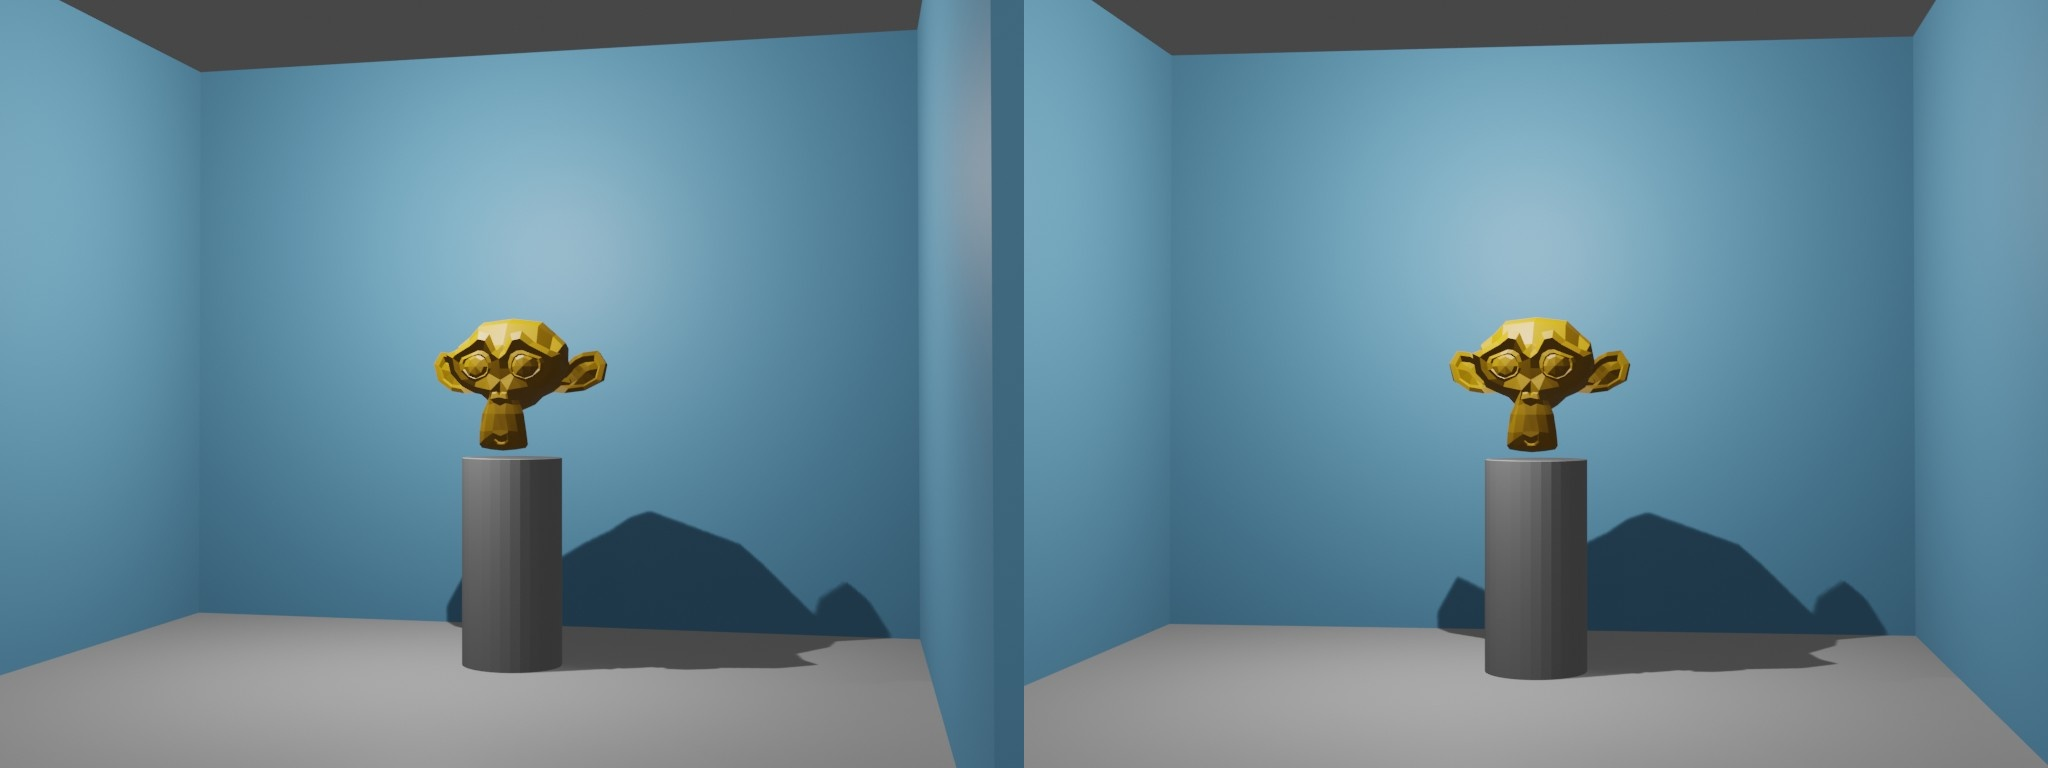
\includegraphics[width=\textwidth]{img/experiment2_environment_comparison_2.jpg}
		\caption{An example training image generated with the help of Blender.}
	\end{subfigure}
	~ 
	\begin{subfigure}[t]{\textwidth}
		\centering
		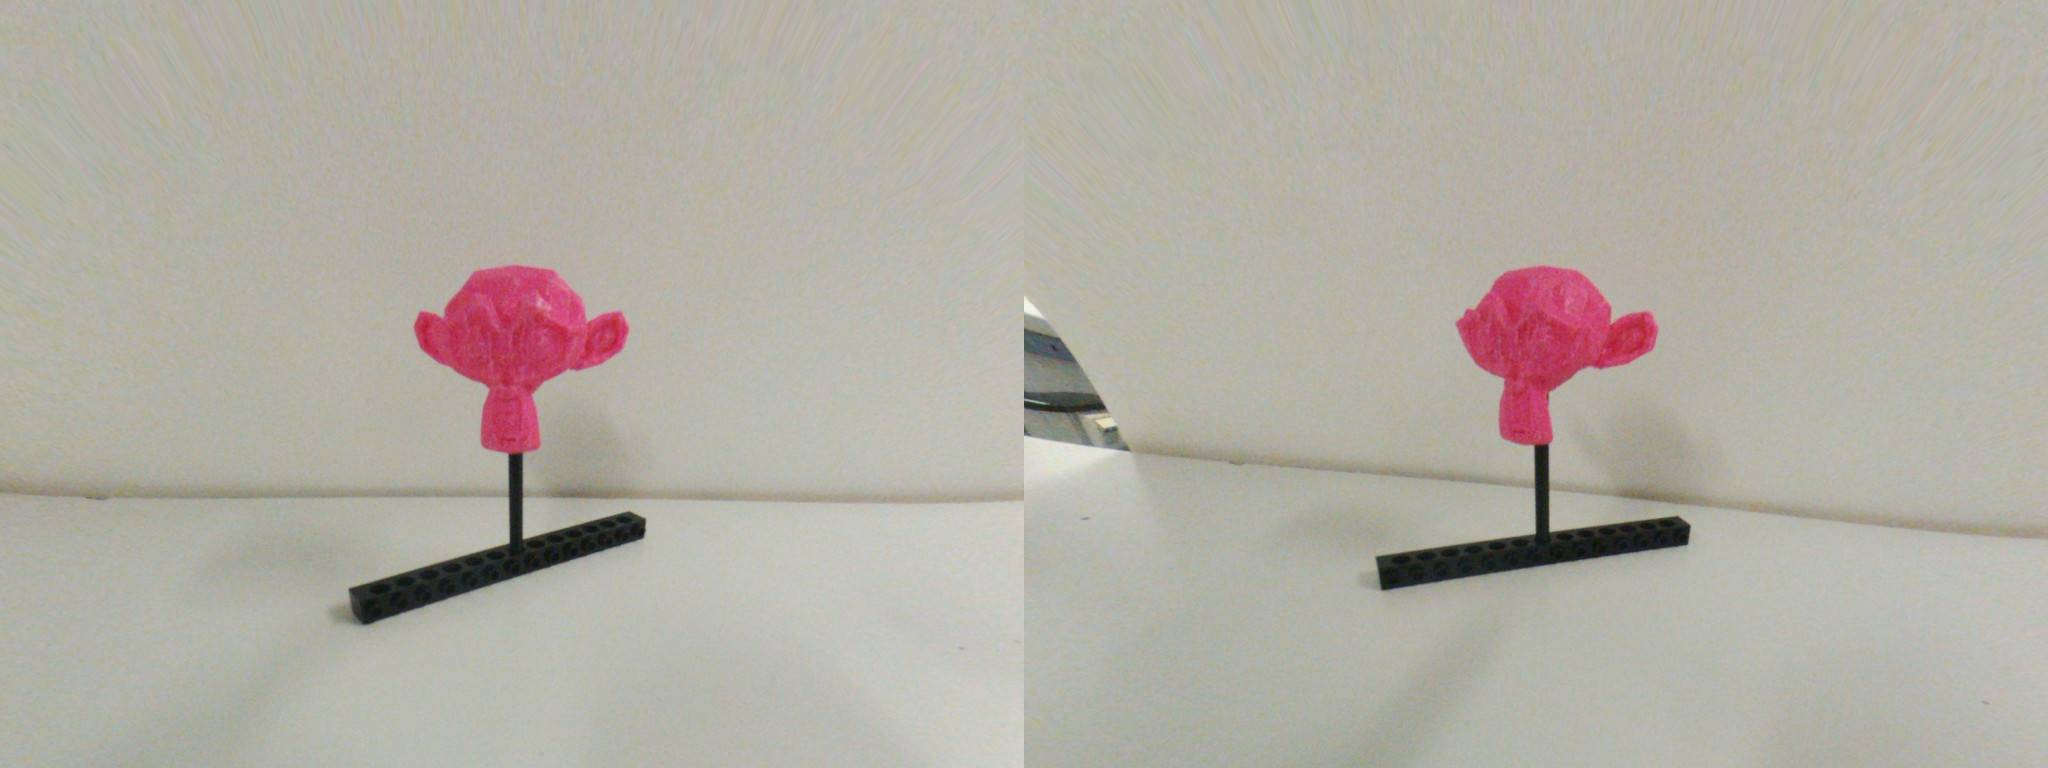
\includegraphics[width=\textwidth]{img/experiment2_environment_comparison_1.jpg}
		\caption{The two modified images of the 3D printed monkey head taken with the Parrot Bebop 2.}
	\end{subfigure}
	\caption{Image pairs of the monkey head.}
	\label{pic:experiment2_environment_comparison}
\end{figure*}

\vspace{5mm}
\noindent
\textbf{Author: Ida Hönigmann}

\section{Results}
Because the preparation of the images made with the Bebop Parrot 2 camera was time consuming only one pair of images was tested. The result of the prediction of this image pair was the following:

\begin{lstlisting}[]
images 0 to 1:
prediction - [3.451700 0.146270 -1.12407]    actual - [0.130000 0.030000 0.020000]
\end{lstlisting}

The fact that the prediction is off by more than one meter shows that the neural network was not able to generalise to real images. This could have multiple reasons:

\begin{itemize}
	\item the units of the scenes in Blender could not be compatible with real world units this easily,
	\item the complexity of estimating real world distances could be a more complex problem, than the limited layer neural network build by the authors can solve,
	\item the different colours of the real objects, compared to the ones in Blender, could cause confusion,
	\item the neural network could have been trained for too long (overfitting) or
	\item the missing shadow, due to the different lighting situation could have caused the problem.
\end{itemize}

It is also possible that a completely different circumstance caused the problem, but the authors could not test any hypothesis due to the limited time frame of this work.

\filbreak